\subsection{Analytic solutions}

Following our earlier remarks, we can formally differentiate the equation to obtain a recurrence relation for the derivatives of $u$. If one specifies initial data at $t = 0$, these relations fully determine all the derivatives $\partial_t^k u (0)$. In the case where the non-linearity is analytic, the formal power series for $u$ is the natural candidate for the solution to the initial data problem. 


\begin{theorem}[Cauchy-Kowalevskaya theorem]
	Let $F \in C^\omega (\R^n \to \R^n)$ be analytic, then there exists a unique analytic solution to the initial data problem (\ref{eq:idp}). 
\end{theorem}

\begin{proof}
	By replacing $u$ with $u - u_0$, it is not a loss of generality to prove solve the equation for initial data $u_0 = 0$. Our goal is to obtain an \textit{a priori} estimate on the growth of $\partial_t^m u(0)$ such that the \textit{ansatz}
		\[ u(t) := \sum_{n = 0}^\infty \frac{\partial^n_t u (0)}{m!} t^m \]	
	is shown to be analytic. It would follow by construction and the uniqueness theorem then that $\partial_t u - F(u) \equiv 0$ since the left-hand side is an analytic function which vanishes to every order at $t = 0$. Formally differentiating the equation, it follows from the chain rule and induction that the derivatives of $u$ can be written as a polynomial with non-negative coefficients in the derivatives of $F$ up to order $m - 1$,
		\[ \partial_t^m u = p_m ( F (u),  \nabla F(u), \dots, \nabla^{m - 1} F(u)) \]
	for some $p_m \in \N_0 [\vec x]$. Using the initial data $u(0) = 0$, it follows that $\partial_t^m u (0)$ are fully determined by $\nabla^j F(0)$ up to order $j < m$. Note that the polynomial $p_m$ is determined combinatorially, depending only on the order $m$. To estimate the growth of $\partial_t^m u (0)$, we argue by \textit{analytic majorisation}; non-negativity of the coefficients of $p_m$ imply 
		\begin{equation}
			|\partial^m_t u (0)| \leq \partial^m_t v(0)
			\tag{*}
			\label{eq:major}  
		\end{equation}	
	for any solution to the initial data problem	
		\begin{align*}
			\partial_t v 
				&= G(v) ,\\
			v_{|t = 0}
				&= 0,	
		\end{align*}
	for some analytic $G \in C^\omega (\R^n \to \R^n)$ such that $|\partial^m F_i (0)| \leq \partial^m G_i (0)$. Our strategy will be to choose $G$ such that the auxiliary ODE above is explicitly solvable for analytic $v$. The growth estimates on the power series of coefficients of $v$ also hold for those of $u$ via the majoristion (\ref{eq:major}), completing the proof. To construct $G$, we know from analyticity of $F$ that there exists $r > 0$ such that
		\[ |\nabla^m F(0)| \leq \frac{m!}{r^{m + 1}}. \]
	We construct $G$ such that the $m$-th order derivatives are precisely the right-hand side, namely
		\[  G_i (z_1, \dots, z_n) := \frac{1}{r - z_1 - \dots - z_n}. \]	
	For simplicity, consider the scalar case $n = 1$, the higher dimensional case is similar. By separation of variables, the explicit solution is given by $v(t) = r - r \sqrt{1 - 2t}$, which is clearly analytic in the region $|t| < r/2$. This completes the proof. 
\end{proof}


\subsection{Picard iteration}

	From the strong solution perspective, solving (\ref{eq:idp}) is equivalent to finding a \emph{fixed point} $\Phi_{u_0} (u) = u$ of the integral operator $\Phi_{u_0} : C^0 ([0, T] \to \R^n) \to C^0 ([0, T] \to \R^n)$ defined by 
		\[ (\Phi_{u_0} u)(t) := u_0 + \int_0^t F(u(s)) \, ds. \]
	We will argue by \textit{Picard iteration}. Schematically, we start off with an approximate solution $u_0$, and inductively construct subsequent approximates $u_{n}$ by inputting $u_{n - 1}$ into the integral operator,
		\[ u_n := \Phi_{u_0} (u_{n - 1}) = u_0 + \int_0^t F(u_{n - 1}(s)) \, ds .\]
	These approximate solutions are known as \emph{Picard iterates}, and the goal then is to show that this sequence $\{u_n\}_n$ converges uniformly to some $u$. If this were true, then by continuity of $\Phi_{u_0}$ and construction of the sequence, the limit $u$ would be a fixed point. A sufficient condition is if $\Phi_{u_0}$ is a \emph{contraction}, i.e. Lipschitz continuous with constant $L < 1$, 
	\[ || \Phi_{u_0} (u) - \Phi_{u_0} v||_{C^0[0, T]} \leq L ||u - v||_{C^0[0, T]}. \]
	\begin{figure}[h]
		\begin{center}
			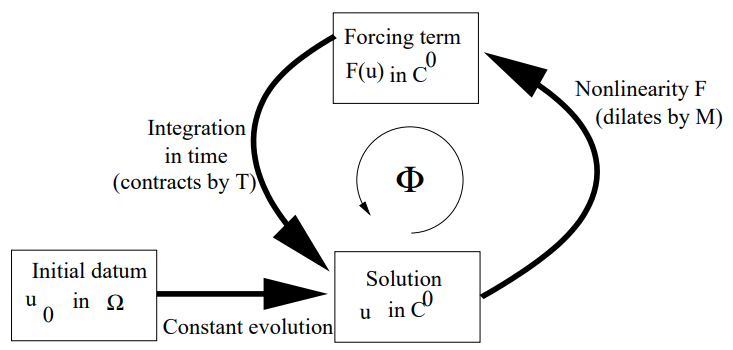
\includegraphics[scale = 0.6]{picard}
			\caption{The strong solution notion says that $u$ is determined by its past via integration in time. Thus for $T \ll 1$, the initial data $u_0$ is a good approximate solution. Iterating these approximations through the operator $\Phi_{u_0}$ converges provided we have some ``gain'' at each stage. }
		\end{center}
	\end{figure}
	
\begin{lemma}[Contraction mapping principle]
	Let $(X, d)$ be a complete non-empty metric space, and let $\Phi : X \to X$ be a contraction on $X$. Then there exists a unique fixed point $u = \Phi(u)$. Furthermore, if $u_0 \in X$ and we construct the sequence $\{u_n\}_n \subseteq X$ iteratively by 
		\[ u_{n + 1} := \Phi(u_n),\]
	then $u_n \to u$. 
\end{lemma}

\begin{proof}
	To show existence, we aim to show that the iterates $\{u_n\}_n$ form a Cauchy sequence. For $n, k \geq 0$, we obtain
		\begin{alignat*}{2}
			 d(u_n, u_{n + k}) 
			 	&= d(\Phi^n (u_0), \Phi^n (u_k))			
			 		&&\\
			 	&\leq c^n d(u_0, u_k) 
			 		&&\\
			 	&\leq c^n \left( d(u_0, \Phi(u_0)) + \dots + d(\Phi^{k - 1} (u_0), \Phi^k (u_0)) \right) 
			 		&&, \\
			 	&\leq 	c^n \sum_{j = 0}^{k - 1} c^j d(u_0, \Phi(u_0))
			 		&& \\
			 	&\leq \frac{c^n}{1 - c} d(u_0, \Phi(u_0))
			 		&&.	
		\end{alignat*}	 
	Since $0 < c < 1$, the above vanishes upon passing the limit $n \to \infty$, proving that the sequence is Cauchy. Since $X$ is complete, we know that there exists a limit $u \in X$. As contractions are continuous, 
		\[ \Phi(u) = \Phi( \lim_{n \to \infty} u_n) = \lim_{n \to \infty} \Phi(u_n) = \lim_{n \to \infty} u_{n + 1} = u.  \]
	To show uniqueness, suppose $v \in X$ is another fixed point, then by definition and the contraction inequality
		\[ d(u, v) \leq cd(u, v), \]	
	which, since $0 < c < 1$, can only hold if $d(u, v) = 0$ i.e. $u = v$. 
\end{proof}

\begin{theorem}[Picard-Lindelof existence theorem]
	Let $\Omega \subseteq \R^d$ be a domain, and suppose $F \in \dot C^{0, 1}_{\loc} (\Omega \to \R^d)$ is locally Lipschitz. For initial data $u_0 \in \Omega$ and $\epsilon \ll 1$, set
		\begin{align*}
			L
				&:= ||F||_{\dot C^{0, 1} (\overline{B_\epsilon (u_0)})} ,\\
			M
				&:= ||F||_{C^{0} (\overline{B_\epsilon (u_0)})}.	
		\end{align*}
	Then for $T < \min (\epsilon/M, 1/L)$, there exists a strong solution $u: [0, T] \to \overline{B_\epsilon (u_0)}$ to the initial data problem (\ref{eq:idp}). 
\end{theorem}

\begin{proof}
	The contraction mapping principle furnishes a solution provided we show that the integral operator $\Phi_{u_0}$ is a contraction mapping on the closed ball $C^0 ([0, T] \to \overline{B_\epsilon (u_0)})$. We first show $\Phi_{u_0}$ maps the desired space into itself: by choice of $T$ and $M$, we have 
		\begin{align*}
			 ||(\Phi_{u_0} u)(t) - u_0||_{C^0 [0, T]} 
			 	&\leq \int_0^T |F(u(s))| \, ds \leq TM \leq \epsilon. 
		\end{align*}
	Next, we show $\Phi_{u_0}$ is a contraction: 
		\[ ||\Phi_{u_0} u - \Phi_{u_0} v||_{C^0 [0, T]} \leq  \int_0^T |F(u(s)) - F(v(s))| \, ds \leq T L ||u - v||_{C^0}, \]
	where $TL < 1$ by construction. This completes the proof.
\end{proof}

\begin{remark}
	A common theme in solving ODEs and more generally PDEs is that we need to exploit some ``smallness'' to get an estimate or iteration to close. In this case, we exploit the time of existence $T$ to ``defeat'' any large oscillations from $F$ which could prevent the iteration from converging. 
\end{remark}


\subsection{Compactness solutions}

Suppose now we only had continuity of the non-linearity $F$ and no control over the Lipschitz norms. We again argue by approximation, this time approximating the equation and showing the corresponding solutions converge via \textit{compactness}, namely 

\begin{lemma}[Arzela-Ascoli theorem]
	Let $(X, d)$ be a compact metric space, and let $\cF \subseteq C(X)$ be a family of continuous functions. Then $\cF$ is pre-compact if and only if 
	\begin{itemize}
		\item $\cF$ is uniformly bounded, that is, $||f||_{C(X)} \lesssim 1$ uniformly in $f \in \cF$, 
		\item $\cF$ is equicontinuous, that is, for every $\epsilon > 0$ there exists a uniform $\delta > 0$ such that $|f(x) - f(y)| < \epsilon$ whenever $|x - y| < \delta$ for all $f \in \cF$.
	\end{itemize}
\end{lemma}

While we can approximate the non-linearity in the uniform topology by Lipschitz functions, there is no uniform control over the Lipschitz constants. Thus, following the proof of the Picard-Lindelof theorem, we cannot quantitatively show the approximate solutions exist on the same time interval existence. We instead turn to a more qualitative argument relying on \textit{continuous induction on time} to show that the solutions do not ``escape'' a ball in arbitrarily small time. 

\begin{lemma}[Bootstrap argument]
	Let $f : [0, T) \to [0, \infty)$ be continuous, and suppose $f(0) \leq C$. Suppose that $f(t) \leq 2C$ implies the stronger bound $f(t) \leq C$, then the stronger bound holds for all time. 
\end{lemma}

\begin{proof}
	We argue by connectedness of the interval $[0, T)$. The set of times $A \subseteq [0, T)$ where $f(t) \leq 2C$ holds is
		\begin{itemize}
			\item non-empty, since $0 \in A$, 
			\item closed, since $f$ is continuous, 
			\item open, since if $t \in A$, then we in fact have the stronger bound $f(t) \leq C$, which by continuity allows us to propagate the weaker bound forward in time $f(t^+) \leq 2C$. 
		\end{itemize}
	Hence $A = [0, T)$. 
\end{proof}

\begin{remark}
	The weaker estimate $f(t) \leq 2C$ is known as a \emph{bootstrap assumption}. Since it in fact implies a stronger bound $f(t) \leq C$, the estimate ``picks itself up by its bootstraps''. 
\end{remark}

\begin{theorem}[Peano's existence theorem]
	Let $\Omega \subseteq \R^n$ be a domain and suppose $F \in C^0_{\loc} (\Omega \to \R^n)$ is continuous. Then for any $u_0 \in \Omega$, there exists a local solution to the initial data problem (\ref{eq:idp}).
\end{theorem}

\begin{proof}
	Assume without loss of generality $u_0 = 0$. There exists $\{ F_k \}_k \subseteq C^\infty (\Omega \to \R^n)$ such that $F_k \to F$ uniformly on compact sets. Smooth functions are locally Lipschitz, so, choosing a small closed ball $\overline{B_\epsilon (0)} \subseteq \Omega$, Picard-Lindelof furnishes local solutions $u_k : [0, T_k) \to B_\epsilon (0)$ to the initial data problems
	\begin{align*}
		\partial_t u_k 	
			&= F_k(u_k), \\
		{u_k}_{|t = 0}		
			&= 0
	\end{align*}
	We claim that there exists a uniform time interval $[0, T] \subseteq \bigcap_k [0, T_k)$ on which $\{u_k\}_k$ exist and are pre-compact. By uniform convergence, there exist uniform constant $M > 0$ such that $|F_k (u)| \leq M$ whenever $|u| \leq \epsilon$. Let $0 < T < \epsilon/(2M + 1)$, we make the bootstrap assumption that $|u_k| \leq \epsilon$ on the interval $[0, T]$. It follows that
		\[ |u_k (t)| \leq \int_0^T |F_k (u_k (s))| \, ds \leq T M \leq \frac\epsilon2 \]
	for all $t \in [0, T]$. The local well-posedness theory allows us to continue the solution, thus by continuous induction on time $u_k$ exists on $[0, \epsilon/(2M + 1)$ and satisfies the uniform bound $|u_k| \leq \epsilon$. Furthermore the equation implies $|\partial_t u_k| \leq M$. This proves $\{u_k\}_k$ is uniformly bounded and equicontinuous, so by Arzela-Ascoli we pass to a subsequence which converges uniformly to a continuous function $u$. As $F_k (u_k (t)) \to F(u(t))$ uniformly, we conclude $u$ is a desired strong solution, i.e. 
		\[ u(t) = \lim_{k \to \infty} u_k (t) = \lim_{k \to \infty} \int_0^t F_k (u_k (s)) \, ds = \int_0^t F (u(s)) \, ds\]
	for all $t \in [0, \epsilon/(2M + 1)]$. 	
\end{proof}


\begin{remark}
	Uniqueness may fail without further assumptions on the regularity of $F$; for example, letting $0 < \alpha < 1$, consider the initial data problem
			\begin{align*}
				\partial_t u 	&= |u|^\alpha, \\
				u_{|t = 0}		&= 0.
			\end{align*}
	Then 
		\begin{equation}
			u (t) = 
				\begin{cases}
					0, 												&\text{if } t \leq t_0, \\
					\left(\frac{1}{1 - \alpha} \right)^{\frac{1}{\alpha - 1}} (t - t_0)^\frac{1}{1 - \alpha}, 	&\text{if } t > t_0,
				\end{cases} \tag{*} \label{eq:nonunique}
		\end{equation}
	is an infinite family of solutions indexed by $t_0 \geq 0$. As a general principle, \textit{sub-linear} forcing terms contribute to non-uniqueness. 
	
	
	\begin{figure}[h]
	\begin{center}
		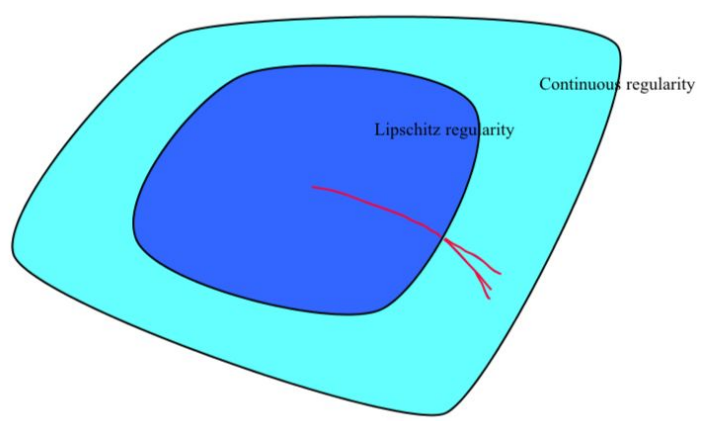
\includegraphics[scale = 0.5]{unique}
		\caption{Uniqueness fails once the solution leaves the regime of Lipschitz regularity. Approaching the boundary can be viewed as a \textit{blow-up criterion}, see Section 5 for details. }
	\end{center}
\end{figure}
\end{remark}

\begin{example}
	Uniqueness breaks down in that the compactness solution depends on the choice of approximation by smooth functions. Let's consider the previous example for $\alpha = \tfrac12$. Fix $t_0 \geq 0$, and define a uniform approximation of $F(u) := |u|^{1/2}$ by Lipschitz functions $F_k : \R \to \R$ by
		\[
			F_k (u) := \left( \max\left\{ |u| - \frac1k, 0 \right\} + \frac{1}{k^2 t_0^2} \right)^{1/2}.	
		\]
	The solutions $u_k : [0, \infty) \to \R$ to the corresponding initial data problems are given by 
		\[ u_k (t) 
			:= \begin{cases}
				\frac{t}{kt_0}, 
					&\text{if } t \leq t_0, \\
				\frac1k - \frac{1}{k^2 t_0^2} + \frac{(t - t_0 + \frac{2}{kt_0})^2}{4}
					&\text{if } t > t_0,
				\end{cases}	
		\]	
	and converge locally uniformly to (\ref{eq:nonunique}). 
\end{example}